%! Date = 18/07/2022

\documentclass[a4paper,11pt,draft=false,bibliography=totoc]{scrartcl} % scrartcl scrreprt scrbook

\usepackage{ebgaramond} % gillius ebgaramond
\usepackage{amsmath}
\usepackage[ngerman]{babel}
\usepackage{relsize}
\usepackage{caption}
\usepackage{tabularx}
\usepackage[newfloat=true]{minted}
\usepackage{pdfpages}
\usepackage[utf8]{inputenc}
\usepackage[automake]{glossaries-extra}
\usepackage[onehalfspacing]{setspace}
\usepackage{graphicx}
\usepackage{csquotes} % dependency of biblatex
\usepackage{biblatex}
\usepackage{xcolor}
\usepackage{newfloat}
\usepackage[section]{placeins} % keep figures near declaration inside Anhang
\usepackage{subcaption}
\usepackage{pifont} % checkmarks
\usepackage{newunicodechar}

% Prüflingsnummer: 144-10013
% Azubinummer: 480513

\newunicodechar{✔}{\ding{52}}

\bibliography{refs}

\setlength{\parindent}{0pt} % disable weird indentation after \begin...\end sections for now
\graphicspath{ {./images/} }

\makeglossaries

\newglossaryentry{Textpassage}
{
    name=Textpassage,
    description={Ein Stück Text aus einer Textdatei. Dabei
            wird sich meist auf eine in der Konfigurationsdatei spezifizierte
            Zieldatei des Programms bezogen.}
}

\newglossaryentry{Zielmuster}
{
    name=Zielmuster,
    description={Ein Element innerhalb der Konfigurationsdatei. Es bezeichnet ein
            Stück Text das einen speziellen \gls{Platzhalter}, den Text \mintinline{bash}{{{value}}},
            enhält. Es wird vom Programm dazu genutzt den genauen Ort der Ziel-\gls{Textpassage}
            innerhalb der Zieldatei zu identifizieren. Das Zielmuster sollte}
}

\newglossaryentry{Platzhalter}
{
    name=Platzhalter,
    description={Ein vordefinierter Text: das englische Wort \mintinline{bash}{value}
            umgeben von doppelten geschweiften Klammern:
            \mintinline{bash}{{{value}}} Das Format des Platzhalters ist an die
            die Template-Engine Template-Engine Jinja2 \cite{jinja2} angelehnt.
            Er ist Teil des \gls{Zielmuster}s das zusätzlich Text vor und nach
            der Ziel-\gls{Textpassage} enthält. Er markiert den Ort der Ziel-\gls{Textpassage}
            relativ zum \gls{Zielmuster} innerhalb der Zieldatei.}
}

\newglossaryentry{Property-Based-Testing}
{
    name=Property-Based-Testing,
    description={Property-Based-Testing bezeichnet eine spezielle Strategie Softwaretests
            zu formulieren. Statt einer Reihe explizit ausformulierter Tests wird eine Regel
            formuliert, welcher das zu testende Programm für automatisch generierte Eingabewerte
            genügen muss.}
}

\glsaddall

\author{
	Prüfungsbewerber: Adrian Schurz\\
	Azubinummer: 480513\\
	Prüfungsnummer: 144-10013\\
	Betreuer: Falk Döring
}
\title{Dokumentation der Projektarbeit zur Ausbildung zum Fachinformatiker für Anwendungsentwicklung}
\subject{Terminal-Config-Manager}
\subtitle{
	CHECK24 Tech Hub und Services GmbH\\
	Tröndlinring 3, 04105 Leipzip
}

\begin{document}

\definecolor{codebg}{rgb}{0.95,0.95,0.95}

\titlehead{\centering
\includegraphics[scale=0.8]{header.png}}
\maketitle
\pagenumbering{gobble}
\newpage

\section{Projektantrag}
\begin{center}
	Diese Seite wird später entfernt.
\end{center}
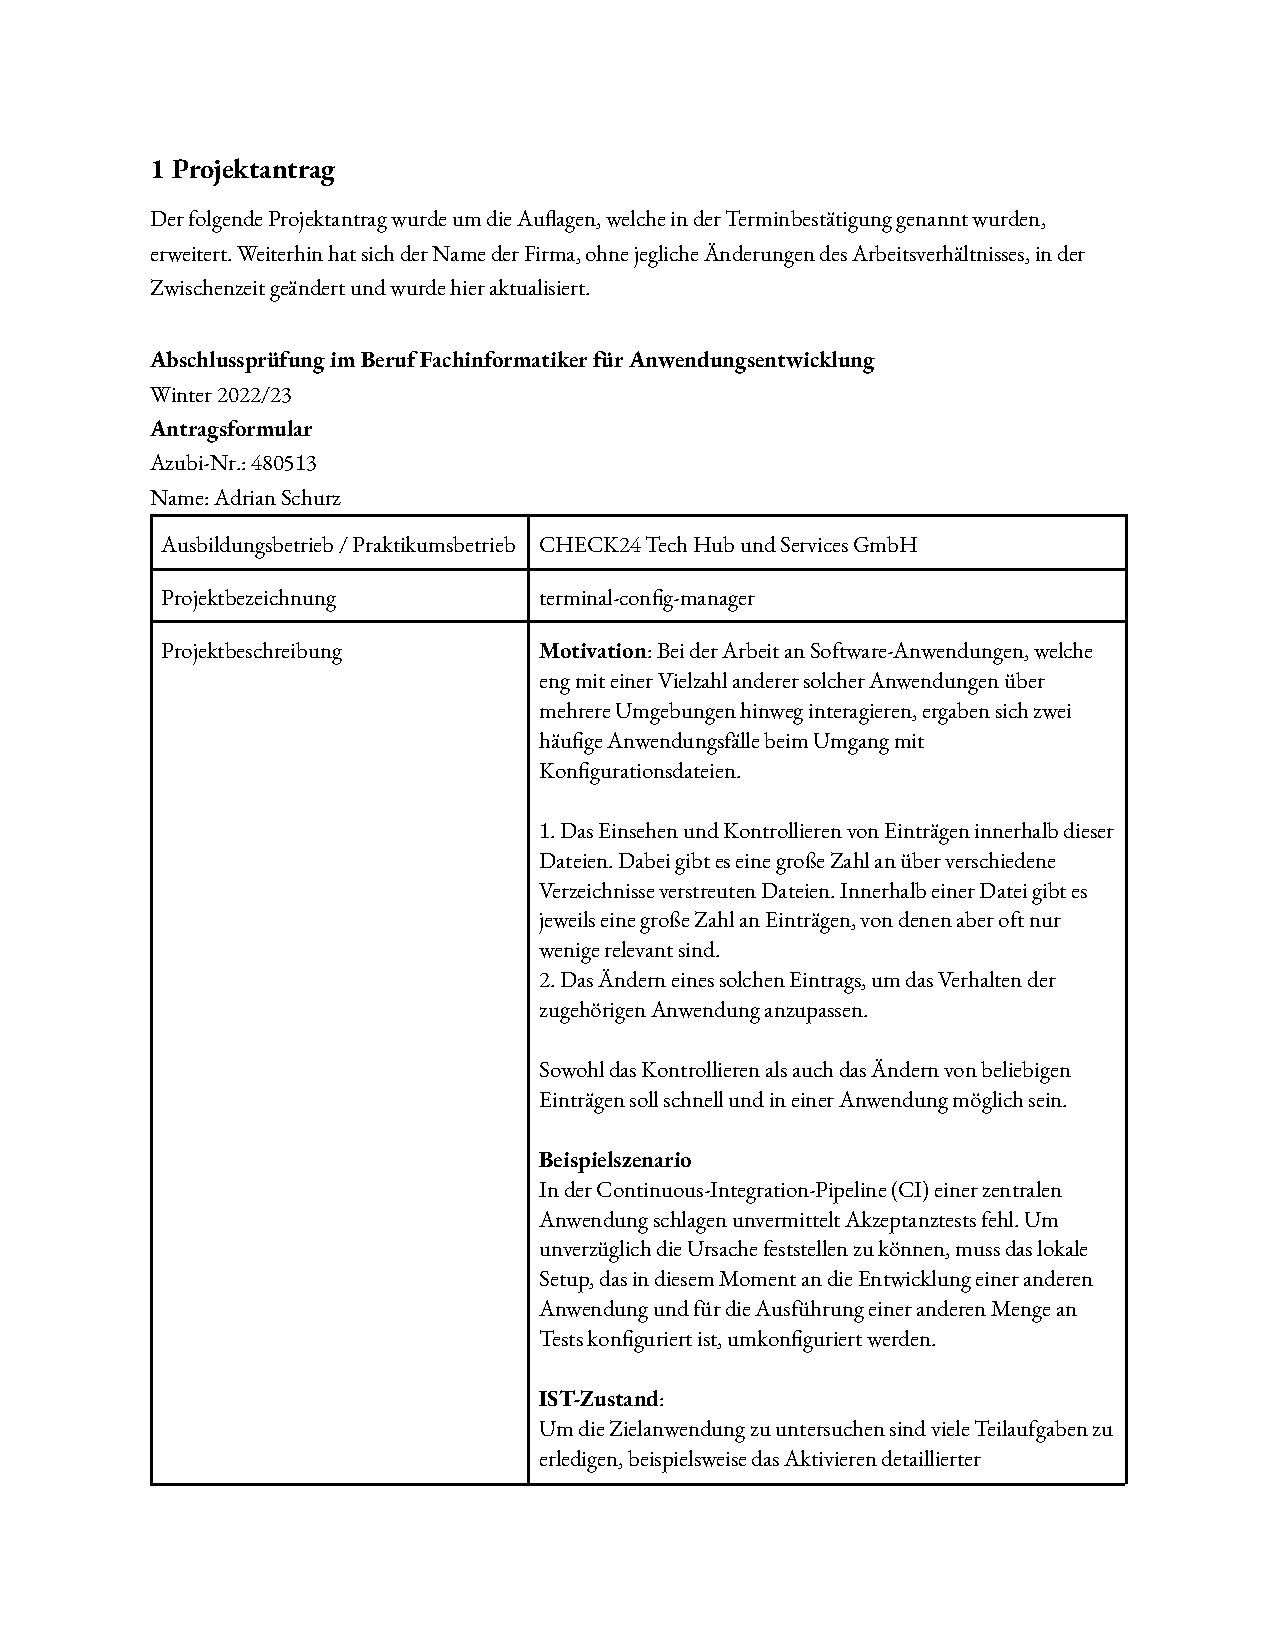
\includepdf[pages={-}]{../projektantrag/projektantrag_final.pdf}

\section{Nachweisblatt}
\begin{center}
	Diese Seite wird später durch den ausgefüllten Zeitnachweis ersetzt.
\end{center}

\newpage
\tableofcontents
\newpage

\pagenumbering{arabic}

\section{Einleitung}
\paragraph{}
Dieses Dokument dient der Dokumentation der betrieblichen Projektarbeit, welche
im Rahmen der Ausbildung zum Fachinformatiker für Anwendungsentwickler durchgeführt
wurde. Die Ausbildung erfolgt unter der Aufsicht der IHK Dresden und im Betrieb
der Check24 Reise Tech Hub und Services GmbH. Der Betrieb ist ebenfalls
Auftraggeber der Projektarbeit.

\paragraph{}
Check24 GmbH ist Betreiber von check24.de, einer Website, auf der verschiedene
Produkte zum Vergleich angeboten werden. Der Auftraggeber betreibt auf dieser
Plattform eine Vergleichsmöglichkeit von Pauschalreisen.

\paragraph{Projektbeschreibung}
Das Projekt dient der Entwicklung eines Software-Tools, das Anwendungsentwickler
bei repetitive Arbeitsabläufen im Umgang mit Konfigurationsdateien unterstützt.
Der Bedarf dafür entstand zwar durch die speziellen Gegebenheiten beim Auftraggeber,
allerdings sind breitere Anwendungsmöglichkeiten denkbar.

\paragraph{Projektziel}
Ziel ist es ein Kommandozeilenprogramm zu entwickeln, welches das Einsehen von
Konfigurationsdateien und das Ändern von Werten innerhalb dieser Dateien vereinfacht.
Die Oberfläche und Nutzung des Programms soll dabei so einfach und übersichtlich
wie möglich gestaltet werden.

\paragraph{Projektbegründung}
Die Zeit die Softwareentwickler in die Bewältigung ihre Aufgaben investieren können
ist aus betrieblicher Sicht eine wichtige, knappe und teure Ressource. Die
Optimierung ihrer Arbeitsprozesse, in diesem Fall die Vereinfachung von repetitiven,
Aufmerksamkeit erfordernden Arbeitsschritten, führt dazu, dass Entwickler ihre
Zeit und Konzentrationsfähigkeit sinnvoller investieren können. Diese Einsparung
kommt wiederum dem Betrieb zugute.

\subsection{Projektabgrenzung}
Das Programm ist vorwiegend als Hilfe für Entwickler gedacht, die eine Vielzahl von
Konfigurationsdateien auf ihrem lokalen Rechner verwalten müssen. Es soll lediglich
per Kommandozeile steuerbar sein und keine zusätzlichen APIs anbieten. Die Einbindung
des Programms in automatische Prozesse, beispielsweise während Deployments, ist
nicht vorgesehen.

\section{Analyse}
\paragraph{}
Der Bedarf für die im Rahmen dieser Projektarbeit erstellte Softwarelösung ergab
sich bei der Arbeit an Software-Anwendungen, welche eng mit einer Vielzahl
anderer Anwendungen und über mehrere Umgebungen hinweg interagieren.

\subsection{IST-Zustand}
Der Großteil dieser Anwendungen besitzt weitläufige Konfigurationsmöglichkeiten
welche ihren Betrieb in verschiedensten Szenarien steuern. Beispiele für
Konfigurationsmöglichkeiten und deren Ausprägungen sind:

\begin{itemize}
    \item Das Loggingverhalten der Anwendung
          \begin{itemize}
              \item Logging gegen die Logverarbeitungssoftware der Produktionsumgebung
              \item Logging gegen eine lokale Instanz der Logverarbeitungssoftware
              \item Logging auf das Dateisystem
              \item Logging mit verschiedenen Logleveln
          \end{itemize}
    \item Die Zieldatenbank der Anwendung \begin{itemize}
              \item Datenbank der Produktionsumgebung
              \item Datenbank der Testumgebung
              \item lokale Datenbank
          \end{itemize}
    \item Die Ausführung von Softwaretests \begin{itemize}
              \item Ausführen von ausschließlich Unittests
              \item Ausführen von Akzeptanztests
              \item Ausführen der Gesamtheit der Tests
              \item Anpassung der Ziel-IP einer weiteren, für die Testausführung
                    notwendigen Anwendung
          \end{itemize}
\end{itemize}

\paragraph{}
Der Kontext der Arbeit an der Software wechselt regelmäßig zwischen Entwicklung und
der Behandlung von Fehlern, welche im Produktions- oder Testbetrieb auftreten.
Um dabei das beobachtete Verhalten der Anwendung korrekt zu interpretieren sind
u.a. zwei Arbeitsschritte häufig zu erledigen:

\begin{itemize}
    \item \textbf{Prüfen} der aktuellen Konfiguration
    \item \textbf{Anpassen} der aktuellen Konfiguration
\end{itemize}

Die Anzahl der an jedem Einzelfall beteiligten Anwendungen und die Anzahl der
Konfigurationsdateien pro Anwendungen führen dazu, dass jeweils viele verschiedene
und weit über das Dateisystem verstreute Dateien relevant sind. Pro Datei und
Einzelfall sind folgende Arbeitsschritte zu erledigen:

\begin{itemize}
    \item Starten der zur Anwendung gehörigen \gls{IDE}
    \item Ermitteln der Konfigurationsdatei
    \item Navigation im Verzeichnisbaum
    \item Öffnen der Datei
    \item Finden des relevanten Eintrags in einer mitunter sehr langen Textdatei
    \item Ermitteln der möglichen Zielwerte
    \item Ändern des Eintrags
    \item Speichern der Datei
\end{itemize}

Diese Einzelschritte, mulipliziert mit der Anzahl an Dateien, stellen eine
große Menge an repetitiven Handlungen dar. Wenn diese erleichtert würden, dann
ließen sich sowohl Zeit und Konzentrationsvermögen einsparen als auch Fehlerpotential
verringern.

\subsection{Soll-Zustand}
Es existiert ein Kommandozeilenprogramm, das übersichtlich eine
Liste anzeigt. Die Liste enthält pro Zeile einen Beschreibungstext
und den aktuellen Wert innerhalb der Zieldatei. Das Programm
erlaubt es, per Tastendruck Zeilen auszuwählen und den
zugehörigen Wert aus einer Menge möglicher Werte auszuwählen.
Wird ein neuer Wert ausgewählt, so wird die dazugehörige
Konfigurationsdatei zum neuen Wert hin umgeschrieben. Sowohl die Zieldateien als
auch die jeweiligen möglichen Werte sind konfigurierbar.
Zusätzlich existieren ausführliche Unit- und Akzeptanztests. \label{Sollzustand}

\subsection{Pflichtenheft} \label{Pflichtenheft}
Dieses Kapitel dient als Pflichtenheft des Projekts. Es enthält, aufbauend auf
der Analyse aus dem vorhergehenden Kapitel eine explizite Auflistung der Anforderungen
an die fertige Software inklusive der Abnahmekriterien. Das Projektumfeld und
sonstige Dopplungen mit den vorangestellten Kapiteln werden dabei ausgespart.

\paragraph{Schnittstellenübersicht}
Das zu erstellende Programm ...
\begin{itemize}
    \item erlaubt die Interaktion mittels Tastatureingaben.
    \item erzeugt Ausgaben in einem Terminal(-emulator).
    \item bietet keine sonstigen Schnittstellen an.
\end{itemize}

\paragraph{Lebenszyklusanalyse}
Das Vorgehen bei der Erstellung des Programms folgt dem Wasserfall-Modell. Die
Auslieferung an den Nutzer erfolgt durch die Bereitstellung eines Zugriffs auf
das Hauptverzeichnis des Projekts. Dies kann beispielsweise über das Hosting des
Git-Projekts per Bitbucket oder Github geschehen. Das Projekt gilt nach
Auslieferung als fertiggestellt, jedoch kann über ebengenannte Hosting-Plattformen
Feedback von Nutzern gesammelt werden. Sollten Softwarefehler durch Nutzer
entdeckt werden, dann werden diese so bald wie möglich beseitigt. Ebenfalls
denkbar ist eine Wandlung des Projekts in ein Open-Source-Projekt. Das hätte zur
Folge, dass Fehler der Software in Kollaboration mit Nutzern und auch durch die
Nutzer selbst behoben werden können.

\paragraph{Funktionale Anforderungen}
Das Programm ...
\begin{itemize}
    \item lässt sich von der Kommandozeile aus starten.
    \item erlaubt die Konfiguration der Menge an Zieldateien.
    \item erlaubt die Konfiguration der zu ändernden Werte pro Zieldatei.
    \item kann über eine Datei im YAML-Format konfiguriert werden.
    \item erlaubt mehrere gängige Pfade für Konfigurationsdateien unter Linux.
    \item zeigt vom Start bis zum Beenden des Programms pro Zieldatei eine Textzeile an.
    \item zeigt pro Textzeile die zur Zieldatei gehörige Beschreibung und den aktuellen Wert an.
    \item hebt die aktuell markierte Zeile sichtbar hervor.
    \item erlaubt die Auswahl einer Zeile mit den Tasten "Pfeil hoch" bzw. "Pfeil runter"
    \item erlaubt die Auswahl eines neuen Werts innerhalb Zieldatei der markierten
          Zeile mit den Tasten "Pfeil links" und "Pfeil rechts".
    \item schreibt bei Auswahl eines neuen Werts diesen in die Zieldatei und ersetzt
          damit ausschließlich den vorherigen Wert.
    \item zeigt zu jeder Zeit am unteren Rand des Terminals Hinweise zur Nutzung
          des Programms an.
    \item informiert den Nutzer im Falle einer Fehlkonfiguration.
    \item informiert den Nutzer im Falle eines fehlerhaften Aufrufs des Programms.
    \item lässt sich mit der Taste "q" beenden und kehrt anschließend zur Kommandozeile zurück.
\end{itemize}

\paragraph{Nichtfunktionale Anforderungen}
Das Programm ...
\begin{itemize}
    \item lässt sich auf Debian- und Arch-Linux-Betriebssystemen über die gängigen
          Paketmanager installieren.
    \item ist in seiner Funktionalität mit Unit- und Akzeptanztest abgedeckt.
    \item ist mit ausführlichen Quellcodekommentaren versehen.
    \item ist mit einer navigierbaren Moduldokumentation im HTML-Format versehen.
\end{itemize}

\paragraph{Abnahmekriterien}
Im Projektverzeichnis wird
\begin{minted}[bgcolor=codebg]{bash}
    stack test
\end{minted}
und damit alle automatisierten Tests ausgeführt. Alle Tests müssen erfolgreich
sein. Desweiteren wird jeder Punkt unter "Funktionale Anforderungen" und
"Nichtfunktionale Anforderungen" händisch geprüft.

\paragraph{Lieferumfang}
Das Programm wird als vollständiges Git-Repository, zusammen mit dem Quellcode,
Moduldokumentation, der ausführbaren Datei und installierbaren Linux-Paketen
ausgeliefert.

\section{Technologie}
\subsection{Kriterien}
\paragraph{}
Für dieses Projekt bieten sich grundsätzlich alle gängigen Programmiersprachen
an. Während der Umsetzung soll ausgewählten Aspekten der Softwareentwicklung
gesonderte Aufmerksamkeit zukommen.

\paragraph{Korrektheit und Laufzeitstabilität} Es soll auf technischem Weg zum
Einen sichergestellt werden, dass sich das Programm zu jedem Zeitpunkt erwartungsgemäß
und korrekt verhält und zum Anderen, dass Fehlerzustände zur Laufzeit so weit
wie möglich ausgeschlossen werden.

\paragraph{}
Als hauptsächliche Wege dies zu erreichen werden folgende Ansätze gewählt:

\begin{itemize}
    \item Wahl einer Programmiersprache mit strenger Typisierung
    \item Wahl einer kompilierten Programmiersprache mit vergleichsweise starken
          Garantien zum Laufzeitverhalten
    \item Einbeziehung von \gls{Property-Based-Testing} \cite{property-based-testing} in das Konzept der Softwaretests
\end{itemize}

\paragraph{Ausführliche, vom Quellcode abgeleitete Moduldokumentation}
Neben der Projektdokumentation soll eine Dokumentation der einzelnen
Softwaremodule entstehen. Um dem Problem zu begegnen, dass Dokumentation und
Quellcode im Laufe der Entwicklung auseinanderlaufen soll die Moduldokumentation
direkt aus den Quellcodekommentaren generierbar sein.

\subsection{Auswahl}
Als Programmiersprache und Build-System wurden auf Basis der obengenannten Ziele
Haskell \cite{haskell} und Stack \cite{stack} gewählt.

\paragraph{}
Stack bietet neben seiner Hauptaufgabe die Software-Abhängigkeiten des Projekts
zu verwalten und den Buildvorgang zu steuern die Möglichkeit Moduldokumentation
im HTML-Format anhand der Quellcodestrukur und der Quellcodekommentare generieren
während Haskell eine typsichere, kompilierte Programmiersprache mit Unterstützung
für \gls{Property-Based-Testing} darstellt.

\section{Projektplanung}

\subsection{Zeit}
Die geplante Umsetzungsdauer beträgt ca. 70 Stunden und ist folgendermaßen
gegliedert.

\begin{center}
    \begin{tabular}{ |c|c| }
        \hline
        \textbf{Projektphase} & \textbf{geplante Zeit (h)} \\ \hline
        Konzeption            & 10                         \\
        Technologiewahl       & 3                          \\
        Einrichtung           & 2                          \\
        Implementierung       & 30                         \\
        Qualitätssicherung    & 15                         \\
        Dokumentation         & 10                         \\ \hline
        \textbf{Gesamt}       & \textbf{70}                \\
        \hline
    \end{tabular}
\end{center}

\subsection{Ressourcen}
\paragraph{}
Hier werden alle zur Fertigstellung des Projekts verwendeten Ressourcen, sowohl
Hardware- als auch Software- und Personalressourcen, aufgelistet.

\begin{itemize}
    \item Hardware \begin{itemize}
              \item Lenovo Thinkpad P52
          \end{itemize}
    \item Software \begin{itemize}
              \item Arch Linux (Betriebssystem) \cite{arch}
              \item Stack (Buildsystem) \cite{stack}
              \item GHC (Compiler) \cite{ghc}
              \item Git (Versionskontrolle) \cite{git}
              \item Haddock (Generierung der Moduldokumentation) \cite{haddock}
              \item Graphmod (Graphgenerierung, Modulabhängigkeiten) \cite{graphmod}
              \item Visual Studio Code (Codeeditor) \cite{vscode}
              \item \TeX -Live (Projektdokumentation) \cite{texlive}
          \end{itemize}
    \item Personal \begin{itemize}
              \item Softwareentwickler zur Umsetzung
              \item Softwareentwickler zur Qualitätskontrolle
          \end{itemize}
\end{itemize}

\subsection{Design}
\paragraph{Nutzerinteraktion}
Für die Art der Benutzerinteraktion des Programms sind mehrere Ansätze denkbar.
Beispielsweise könnte das Programm mit jeweils verschiedenen, aufeinanderfolgenden
Befehlen von der Kommandozeile aus aufgerufen werden wie in Abb. \ref{simple-gui-example}
dargestellt. Alternativ könnte das Program, wie in Abb. \ref{graphical-gui-example} skizziert,
mit einer kompletten, grafischen Oberfläche versehen werden.

\paragraph{}
Als pragmatischer, einfacher und funktionaler Ansatz wurde ein Mittelweg gewählt
bei dem eine Konsolenanwendung beim Start alle einzelnen konfigurierten
Zielwerte auf jeweils einer Zeile darstellt, geöffnet bleibt und auf Tasteneingaben
wartet um entweder eine seiner Funktionen auszuführen oder beendet zu werden (siehe Abb. \ref{post-start}
im Kapitel \ref{Kundendokumentation} - Kundendokumentation).


\begin{figure}
    \caption{Nutzerinteraktion mit aufeinanderfolgenden Befehlen}
    \label{simple-gui-example}
    \begin{minted}[bgcolor=codebg]{bash}
        >_ terminal-config-manager show
    
        1 Anwendung a mit Wert -> b
        2 Anwendung c mit Wert -> d
    
        >_ terminal-config-manager change 2
    
        1 Anwendung a mit Wert -> b
        2 Anwendung c mit Wert -> e
    \end{minted}
\end{figure}

\begin{figure}
    \caption{Nutzerinteraktion über eine grafische Oberfläche und Buttons, skizzenhaft}
    \label{graphical-gui-example}
    \centering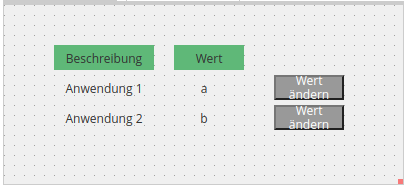
\includegraphics[scale=0.6]{gui-example.png}
\end{figure}

\paragraph{Softwaredesign}
Jeweils funktional zusammengehörige Teile des Quellcodes wurden so gut wie möglich
von anderen Teilen separiert. Die hauptsächliche Organisationsebene bilden dabei
Module, die sich in jeweils einer Quellcodedatei befinden. Beispielsweise ist dadurch
Programmcode, der mit der Verarbeitung von Tasteneingaben betraut ist, im Modul

\begin{minted}[bgcolor=codebg]{bash}
    src/UserInterface/Input.hs
\end{minted}

lokalisiert. Programmcode, welcher mit dem Dateisystem interagiert, dagegen
hier:

\begin{minted}[bgcolor=codebg]{bash}
    src/Infrastructure/FileModification.hs
\end{minted}

Den einzelnen Modulen übergeordnet befindet sich eine Organisationsebene, welche
versucht einem möglichen Ansatz aus dem Kontext des Domain-Driven-Design \cite{domain-driven-design} gerecht
zu werden. Dabei werden Teile des Programmcode in verschiedene Gruppen organisiert,
beispielsweise \textbf{Application}, \textbf{Domain}, \textbf{Infrastructure} und \textbf{Userinterface}, und es wird
darauf geachtet, dass Abhängigkeiten zwischen Modulen dieser Gruppen stets in
eine bestimmte Richtung zeigen. Wenn dieses Schema eingehalten wird, dann können
Probleme, wie zyklische Abhängigkeiten oder schlecht erweiterbare Module, reduziert
oder ganz vermieden werden. Das angestrebte Schema ist dem Buch Domain-Driven-Design \cite{domain-driven-design}
entnommen und ist in Abb. \ref{domain-driven-design-layers} im Angang dargestellt.
Zum Vergleich wurden die tatsächlichen Modulabhängigkeiten mit Unterstützung von
Softwaretools \cite{graphmod} \cite{xdot} ausgelesen und in einem Graphen dargestellt.
In Kapitel \ref{domain-driven-design-result} - Ergebnisdiskussion wird ein Vergleich
angestellt.

\subsection{Projektorganisation}
Die Hauptelemente der Verzeichnisstruktur des Projekts sind wie folgt organisiert.

\begin{minted}[bgcolor=codebg]{text}
    \src
    \test
    \doc
    \distribution
    \bin
    \tool
    package.yaml
    README.md
\end{minted}

Die Verzeichnisse enhalten dabei in der angezeigten Reihenfolge

\begin{itemize}
    \item Quellcode des des Programms
    \item Quellcode der Unit- und Integrationstests
    \item generierte Moduldokumentation und Projektdokumentation
    \item Skripte um Softwarepakete für verschiedene Betriebssysteme zu erstellen
    \item kompilierte, ausführbare Dateien
    \item Hilfsskripte, z.B. zur Generierung des Modulabhängigkeitsgraph
\end{itemize}

\paragraph{}
Die Datei \mintinline{bash}{package.yaml} enthält die für Stack notwendigen Metadaten,
beispielsweise Deklarationen der verwendeten Softwarebibliotheken und Konfiguration
des Buildprozesses.

\paragraph{}
Die Datei \mintinline{bash}{README.md} enthält eine kurze Beschreibung des
Programms und eine Nutzungsanleitung zusammen mit offenen Aufgaben und
Zusatzinformationen.

\section{Umsetzung}

\subsection{Einrichtung}
\paragraph{}
Es wurde der zur Entwicklung im Tagesgeschäft bei Check24 bereitgestellte Laptop
für das Projekt genutzt auf dem bereits ein Linux-Betriebssystem installiert war.
Auch die genutzte \gls{IDE} war bereits aufgrund anderer Projekte vorinstalliert.
Lediglich die \LaTeX-Entwicklungsumgebung und Details der Build-Umgebung mussten
speziell für dieses Projekt konfiguriert werden.

\paragraph{}
Zu diesem Zweck wurde über das Betriebssystem \TeX-Live \cite{texlive} installiert
und ein Plugin für die \gls{IDE} \cite{latex-workshop}. Die Buildumgebung
wurde so konfiguriert, dass bei jedem Speichern einer Datei das Programm kompiliert wird,
sämtliche Softwaretests ausgeführt werden, sowohl die Moduldokumentation als auch
der Graph der Modulabhängigkeiten neu generiert wird und Tools zur Formatierung
und statischen Codeanalyse ausgeführt werden.

\subsection{Entwicklung}
TODO

\subsection{Dokumentation}
Das Projekt wurde sowohl auf Quellcodeebene zum Zwecke der Weiterentwicklung als
auch für Nutzer bzw. Kunden dokumentiert (siehe Kapitel \ref{Kundendokumentation} - Kundendokumentation).

\paragraph{Code- und Moduldokumentation}
Jedes Modul und jede Deklaration im Code ist mit Codekommentaren versehen wie in
den Abbildungen \ref{codecomment-module} und \ref{codecomment-declaration} darstellt.
Anhand dieser Informationen wird mittels Haddock \cite{haddock}, während des Buildprozesses,
eine navigierbare und übersichtliche Moduldokumentation im HTML-Format erstellt,
die sowohl die Module des Programms selbst als auch die der verwendeten Softwarebibiliotheken
beschreibt und im Projektverzeichnis unter \mintinline{bash}{/doc/generated}
abgelegt ist.

\begin{figure}
    \caption{Beispiel eines Modul-Codekommentars}
    \label{codecomment-module}
    \begin{minted}[bgcolor=codebg]{haskell}
-- Module      : FileSynchronization
-- Description : Expose a function which, for a given config
--   item, will read the corresponding file and determine the
--   current value as it would be identified by the pattern.
-- Copyright   : (c) Adrian Schurz, 2022
-- License     : MIT
-- Maintainer  : adrian.schurz@check24.com
-- Stability   : experimental
...
    \end{minted}
\end{figure}

\begin{figure}
    \caption{Beispiel eines Deklarations-Codekommentars}
    \label{codecomment-declaration}
    \begin{minted}[bgcolor=codebg]{haskell}
-- | A function to change the cursor position to point at the
--   next item.
selectNextItem :: AppState -> AppState
...
    \end{minted}
\end{figure}

\paragraph{Projektdokumentation}
Die Dokumentation der Projektarbeit selbst erfolgt mittels \LaTeX \cite{latex} und
wird im \gls{PDF}-Format exportiert. Alle Quelldateien für dieses Dokument sind
ebenfalls im Projektverzeichnis unter \mintinline{bash}{/doc/azubi-project/projektdokumentation}
auffindbar.

\subsection{Qualitätssicherung}
Zur Qualitätssicherung dienten hauptsächlich Unittests, inklusive \gls{Property-Based-Testing},
und händische Tests.

\paragraph{Unittests}
Ein Beispiel für einen Unittest ist in Abb. \ref{unit-test} gegeben. Damit wird
pro Test die Ausgabe einer Funktion für einen speziellen Eingabewert mit einem
korrekten Ausgabewert verglichen. Diese Art des Testens einzelner Codesegmente ist
sinnvoll, aber aufgrund der beschränkten menschlichen Kreativität nicht besonders
gut geeignet um Grenzfälle mit besonders großen, besonders absurden oder anderweitig
unerwarteten Eingabewerten zu ausfindig zu machen.

\begin{figure}
    \caption{Beispiel eines Unittests, aus Platzgründen mit ... eingekürzt und inklusive
        der Ausgabe bei Ausführung (unterhalb des Pfeils)}
    \label{unit-test}
    \begin{minted}[bgcolor=codebg]{text}
describe "changing the element at a certain index inside of a list" $ do
  it "given a valid index ... apply it at the appropriate index" $
    let someList = [1, 2, 3]
        someFunction = (*) 2
        validIndex = 1
    in changeNthElement validIndex ... someList `shouldBe` [1, 4, 3]

                                ↓

changing the element at a certain index inside of a list
    given a valid index ... apply it at the appropriate index [✔]
    \end{minted}
\end{figure}

\paragraph{\gls{Property-Based-Testing}}
Um die obengenannte Schwäche von reinen Unittests auszugleichen wurden zusätzlich
sogenannte Propertytests verfasst, welche mit einer großen Anzahl von zufällig generierten
Eingabewerten bestimmte Eigenschaften der Ausgabewerte prüfen. In Abb. \ref{property-test}
ist ein Test illustriert, der sicherstellt, dass die Zieldatei, unabhängig von
sowohl ihrem Inhalt als auch dem konfigurierten \gls{Zielmuster}, unverändert
bleibt wannimmer der aktuelle Wert und der neue Zielwert identisch sind. Zu
jeder Ausführung der Testsuite werden dafür eine große Anzahl zufälliger Dateiinhalte
und Zielmuster generiert und die Funktion damit geprüft.

\begin{figure}
    \caption{Beispiel für \gls{Property-Based-Testing}, aus Platzgründen mit ... eingekürzt und inklusive
        der Ausgabe bei Ausführung einer großen Anzahl automatisch generierter Tests (unterhalb des Pfeils)}
    \label{property-test}
    \begin{minted}[bgcolor=codebg]{text}
describe "modifying a string according to a search pattern ..." $ do
    prop "... old and new values are identical ... content unchanged" $
        \tva pat cont -> modify tva tva pat cont == cont

                                ↓

modifying a string according to a search pattern ...
    given that the old and new values are ... content unchanged [✔]
        +++ OK, passed 1000 tests.
    \end{minted}
\end{figure}

\paragraph{Akzeptanztests}
Bestimmte Klassen von Softwarefehlern lassen sich allein mit Unittests nicht
zuverlässig auschließen. Für die umfänglichste Überprüfung der Software sind
Tests, welche die Ausführung des kompilierten Programms, inklusiver simulierter
Nutzerinteraktion, prüfen, von hohem Wert. Es wurde versucht mit Mitteln des
Unittesting in Bash \cite{bats} , virtualisierten Betriebssystemen \cite{virtualbox} \cite{docker}
bzw. \gls{Terminalemulator}en und Tools zur Emulation von Tastatureingaben \cite{xdotool} \cite{ydotool}
solche Test zu realisieren. Das Ergebnis ist in Kapitel
\ref{Testabdeckung} - Testabdeckung dokumentiert. Akzeptanztests, welche nicht
automatisiert durchgeführt werden konnten, wurden regelmäßig händische Tests des
kompilierten Programms auf dem Entwicklungsrechner durchgeführt. Ab einem
gewissen Zeitpunkt während der Entwicklung befand sich das Programm bereits in einem nutzbaren
Zustand. Es wurde vom Entwickler selbst von da an produktiv eingesetzt was,
ähnlich dem Konzept des \gls{Betatesting}s, eine praktisch wertvolle, wenn auch wenig rigorose,
Testabdeckung ermöglicht hat.

\section{Ergebnisdiskussion}

\subsection{Funktionalität}
Die Hauptfunkionalität des Programms wurde erfolgreich umgesetzt und es wird von
mir selbst bereits genutzt. Das Programm arbeitet seither wie erwartet,
ist konfigurierbar und informiert mit lesbaren Nachrichten im Falle eines Fehlers.
Ein weiteres Feature wäre jedoch wünschenswert, die Fähigkeit des Programms mit
schreibgeschützten Zieldateien umgehen zu können und in diesem Fall eine
sudo-Passwortabfrage auszulösen. Letzteres ist nicht Teil der
usprünglichen Anforderungen und wird daher erst zukünftig umgesetzt.

\subsection{Domain Driven Design}
Das Ziel die Abhängigkeiten der einzelnene Softwaremodule untereinander einem
mit dem Domain-Driven-Design kompatiblen Schema folgend zu organisieren ist mit
einer Ausnahme geglückt. Im Anhang, Abb. \ref{domain-driven-design-layers}, sind Module
der Applikationsebene abhängig von Modulen des User-Interface. Das verwendete
\gls{GUI}-Framework, Brick, führt durch sein Interface allerdings zu einem Muster bei
dem diese Abhängigkeit umgekehrt ist. Letzteres wird deutlich beim Vergleich des Schemas mit den
tatsächlichen Modulabhängigkeiten (siehe Abb. \ref{module-dependency-graph} im Anhang).
Dieser Umstand stellt für den Moment eine vernachlässigbare Designschwäche dar die ohne weitere
Konquenz ist. Aus diesem Grund erhielt die Aufgabe dies zu beheben eine niedrige
Priorität und steht vorerst noch aus. Alle sonstigen Module halten das angestrebte
Schema ein.

\subsection{Moduldokumentation}
Das Ziel die Moduldokumentation ständig, während des Buildprozesses, aktuell zu
halten ist teilweise geglückt. Im Projektverzeichnis liegt die ausführliche Moduldokumentation
einschließlich jener der eingebundenen Softwarebibliotheken im HTML-Format vor.
Auszüge davon sind in den Abbildungen \ref{module-doc-index} und \ref{module-doc-state} dargestellt.
Allerdings gibt es seit wenigen Tagen bei neueren Versionen des Buildsystems Stack \cite{stack}
und des Generierungstools Haddock \cite{haddock} eine Inkompatibilität. Bis diese
in diesen Projekten behoben und veröffentlicht ist, ist die in diesem Projekt hinterlegte
Moduldokumentation nicht aktuell. Es ist zu erwarten, dass dieses Problem in naher
Zukunft seitens der Entwickler der beiden Tools behoben wird.

\subsection{Testabdeckung}
Die Abdeckung der Funktionalität des Programms auf Unittest-Ebene ist, besonders
dank der Verwendung von \gls{Property-Based-Testing} \cite{property-based-testing}
zufriedenstellend.

\paragraph{}
Eines der angestrebten Ziele war jedoch neben ausführlichen Unittests ebenso ausführliche
Akzeptanztests bereitzustellen. Dies ist trotz erheblichem Aufwand gescheitert.
Das Programm ist eine Konsolenanwendung, welche auf Tasteneingaben reagiert. Das
bedeutet, dass automatisierte Tests in einer kontrollierten Umgebung Terminal-Emulatoren
starten und ihnen Tasteneingaben simulieren müssen um das Programm zu testen. Je nach
der verwendeten grafischen Benutzeroberfläche des Betriebssystems unterscheiden sich
die Ansätze dies zu erreichen jedoch stark. Es existieren mehr oder weniger gut
gepflegte Open-Source-Softwaretools für die Teilaufgabe der Eingabeemulation. Verschiedene
Kombinationen dieser Tools (xdotool \cite{xdotool} vs ydotool \cite{ydotool}) wurden
mit verschiedenen Displayservern (xorg \cite{xorg} vs. wayland \cite{wayland}),
Betriebssystemen (Ubuntu \cite{ubuntu} vs Arch Linux \cite{arch}), und
Virtualisierungslösungen (virtualbox \cite{virtualbox} vs docker \cite{docker})
evaluiert. Keine der Varianten führte zum Erfolg.

\subsection{Bekannte Fehler}
Es sind zwei Bugs in Software-Abhängigkeiten des verwendeten \gls{GUI}-Frameworks
bekannt, welche mit geringer Häufigkeit das \gls{Rendering} bzw. den Start des Programms
beeinträchtigen. Diese Bugs sind dokumentiert (siehe \cite{bug-vty-startup-crash} und
\cite{bug-vty-terminal-capabilities}). Einer dieser Fehler führt dazu, dass der
aktuelle Wert eines Eintrags weiß statt blau gerendert wird und ist schwer
reproduzierbar (1x ca. pro 50-100 Programmstarts). Der andere Fehler führt zu
einem Crash des Programms beim Start (1x ca. pro 30-50 Programmstarts).


\section{Anhang} \label{Anhang}

\begin{figure}[ht]
    \caption{Generierte Moduldokumentation, Hauptseite}
    \label{module-doc-index}
    \fbox{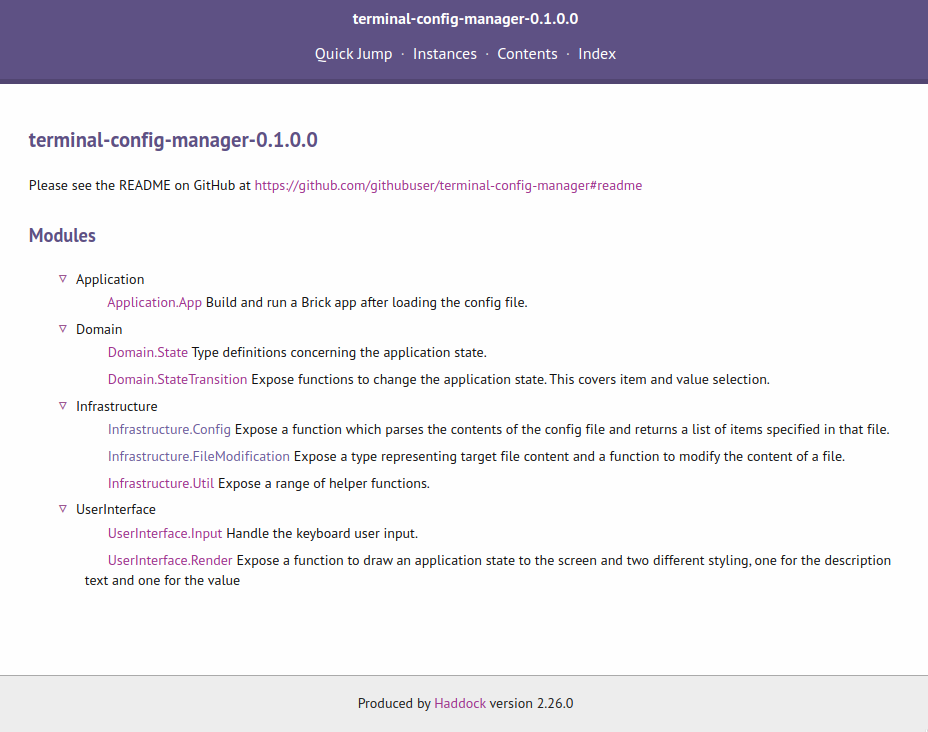
\includegraphics[scale=0.5]{module-documentation-index.png}}
\end{figure}

\begin{figure}[ht]
    \caption{Generierte Moduldokumentation, Domain.State}
    \label{module-doc-state}
    \fbox{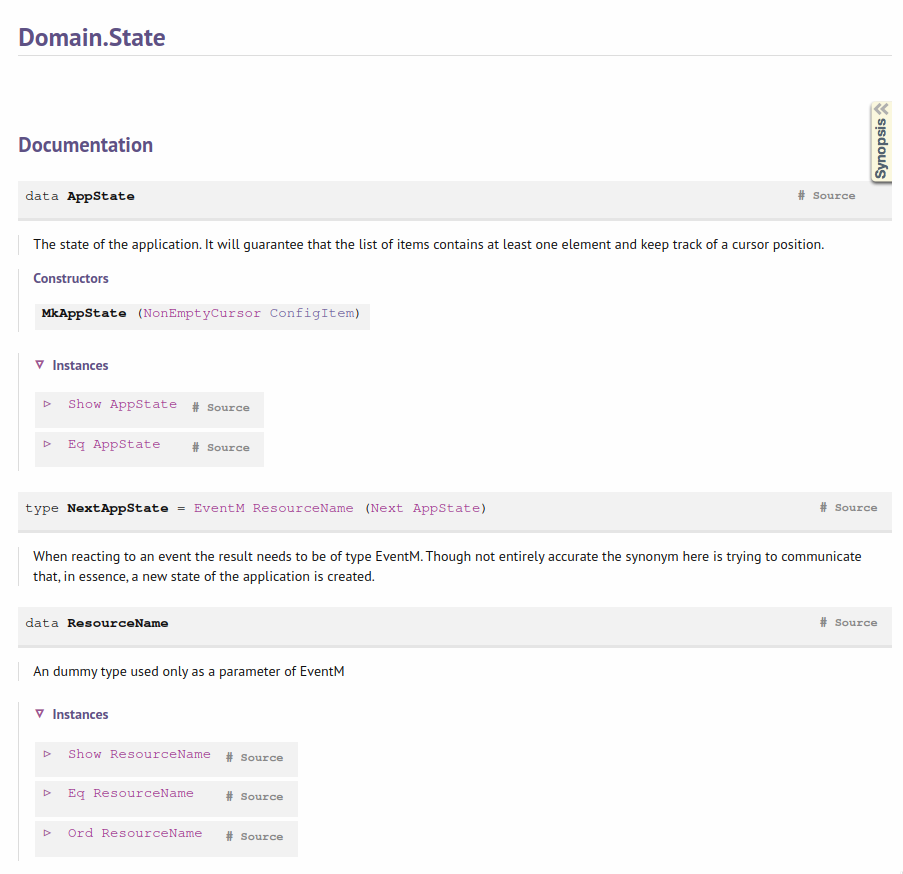
\includegraphics[scale=0.5]{module-documentation-state.png}}
\end{figure}

\begin{figure}[ht]
    \caption{Beispielschema für Modulabhängigkeiten beim Domain-Driven-Design \cite{domain-driven-design}}
    \label{domain-driven-design-layers}
    \centering\fbox{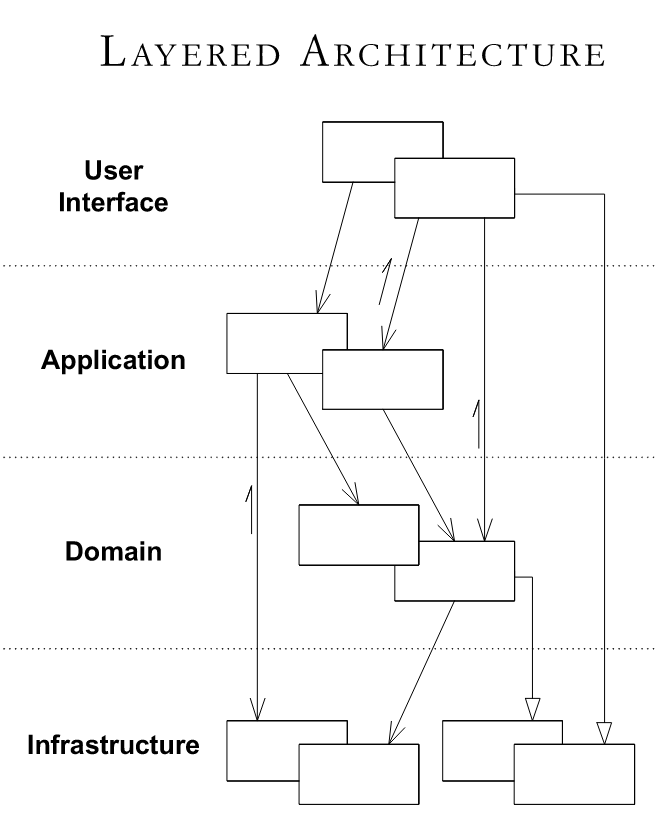
\includegraphics[scale=0.5]{domain-driven-design-layers.png}}
\end{figure}

\begin{figure}[ht]
    \caption{Graph der Modulabhängigkeiten}
    \label{module-dependency-graph}
    \centering\fbox{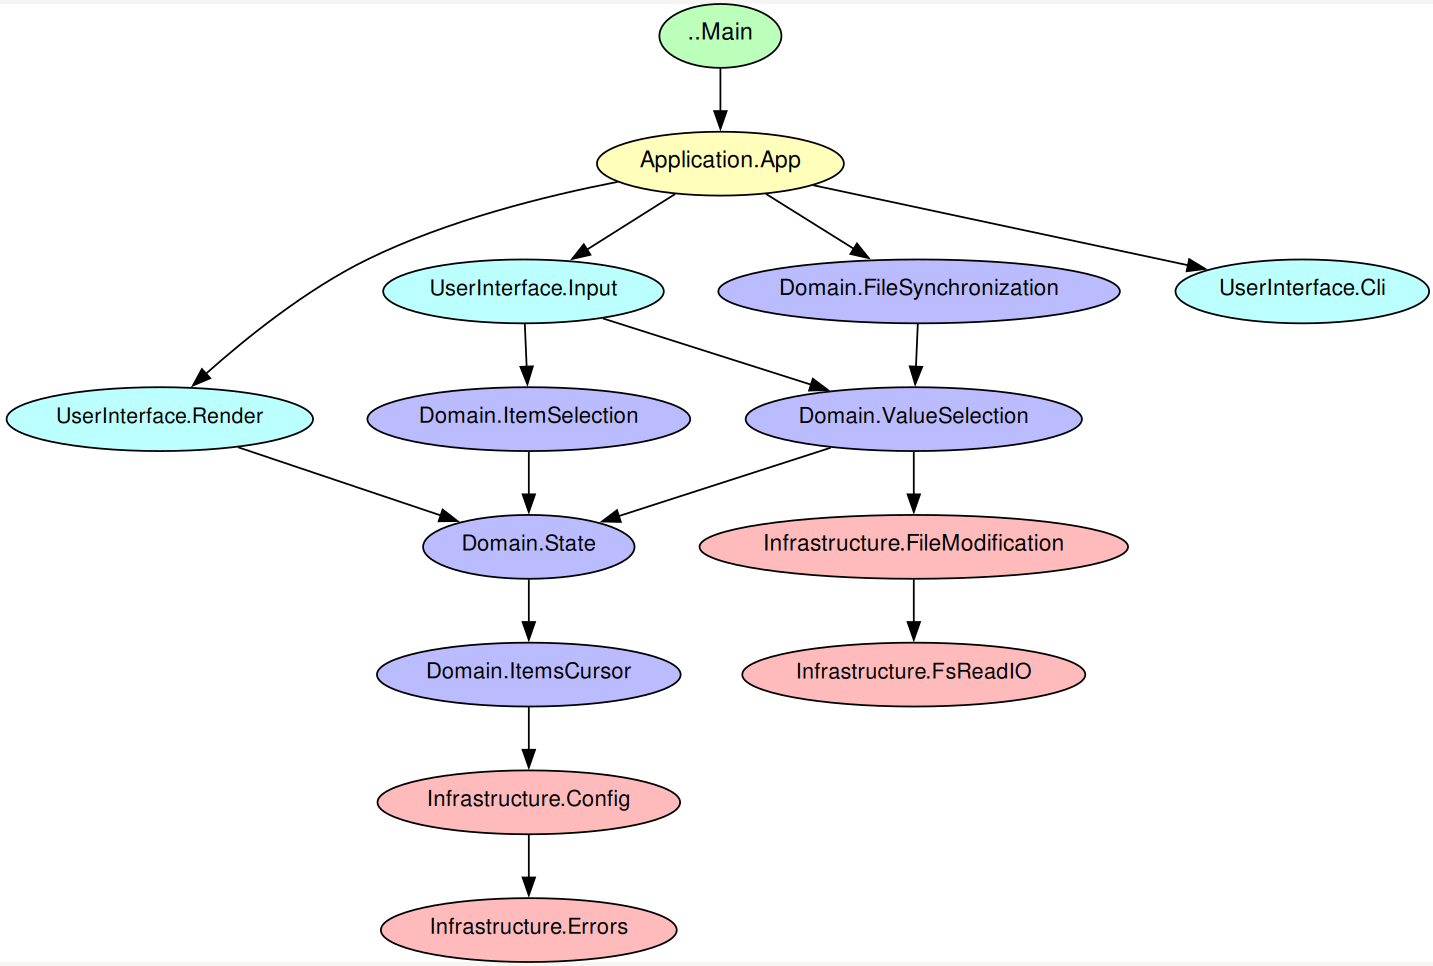
\includegraphics[scale=0.3]{module-dependency-graph.png}}
\end{figure}

\begin{figure}[ht]
    \caption{Ausgabe bei Ausführung der Testsuite}
    \label{test-suite}
    \centering\fbox{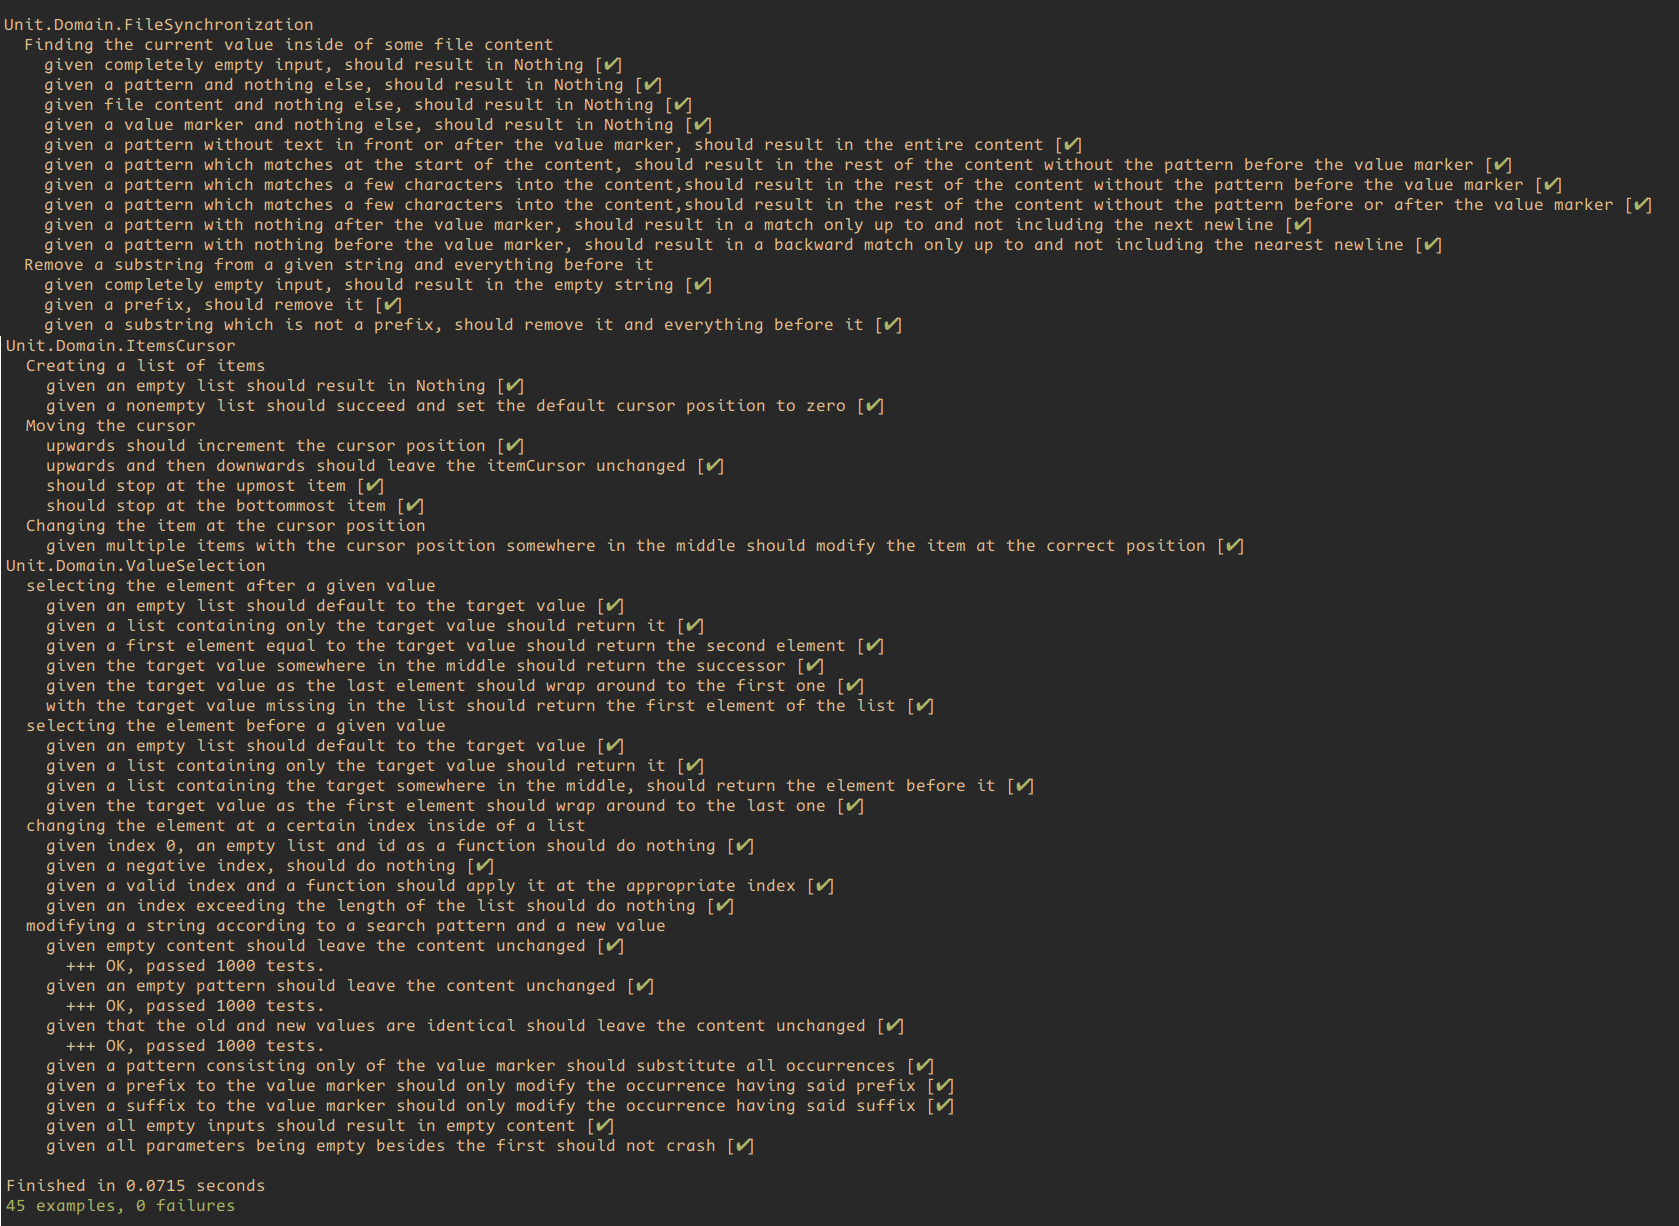
\includegraphics[scale=0.25]{full-test-suite.png}}
\end{figure}

\section{Kundendokumentation} \label{Kundendokumentation}

\subsection{Beschreibung}
Terminal-Config-Manager ist ein Linux-Programm mit welchem
\gls{Textpassage}n innerhalb meherer Dateien schnell zwischen einer Reihe
vorkonfigurierter \gls{Textpassage}n umgeschalten werden können.

Der Hauptanwendungsfall ist die effiziente  Manipulation von
Konfigurationsdateien von Softwareanwendungen, die häufig angepasst
werden müssen.

\subsection{Installation} \label{Installation}
Es wurden vorkonfigurierte Pakete für sowohl ArchLinux\cite{arch}-basierte als auch
Debian\cite{debian}-basierte Betriebssysteme bereitgestellt. Alternativ
kann das Programm auch manuell installiert werden.

\begin{center}
	\textbf{Arch-Linux \cite{arch}, via PKGBUILD Datei und pacman \cite{pacman}}
\end{center}

Im Projektverzeichnis unter

\begin{minted}[bgcolor=codebg]{bash}
	/distribution/arch/PKGBUILD
\end{minted}

befindet sich eine Spezifikationsdatei anhand derer das Softwarepaket
erstellt und anschließend installiert werden kann:

\begin{minted}[bgcolor=codebg]{bash}
	cd distribution/arch
	makepkg
	pacman -U terminal-config-manager-1.0.0-1-x86_64.pkg.tar.zst
\end{minted}

Die Deinstallation erfolgt mittels

\begin{minted}[bgcolor=codebg]{bash}
	pacman -R terminal-config-manager
\end{minted}

\begin{center}
	\textbf{Debian, via .deb Datei und dpkg\cite{dpkg}  bzw. apt\cite{apt}}
\end{center}

Im Projektverzeichnis unter

\begin{minted}[bgcolor=codebg]{bash}
	/distribution/debian/terminal-config-manager.deb
\end{minted}

befindet sich ein Softwarepaket, das mittels \mintinline{bash}{dpkg}
oder \mintinline{bash}{apt} direkt installiert werden kann.

\begin{minted}[bgcolor=codebg]{bash}
	cd distribution/debian
	dpkg --install ./terminal-config-manager.deb
	# apt install ./terminal-config-manager.deb
\end{minted}

Die Deinstallation erfolgt mittels

\begin{minted}[bgcolor=codebg]{bash}
	dpkg --remove terminal-config-manager
	# apt remove terminal-config-manager
\end{minted}

\begin{center}
	\textbf{Alternative, ohne Paketmanager}
\end{center}

Wenn das Programm nicht vom systemeigenen Paketmanager verwaltet werden
soll, dann kann es manuell kompiliert und in einem passenden
Verzeichnis abgelegt werden.

Voraussetzung hierfür ist, dass das Programm \mintinline{bash}{stack} auf dem
System installiert ist.

Im Projektverzeichnis wird mit

\begin{minted}[bgcolor=codebg]{bash}
	stack build --test --copy-bins
\end{minted}

das Programm kompiliert, die Testsuite ausgeführt und die ausführbare Datei im
Projektverzeichnis unter

\begin{minted}[bgcolor=codebg]{bash}
	bin/terminal-config-manager
\end{minted}

abgelegt. Anschließend kann das Programm in ein Verzeichnis kopiert werden, das in die
Systempfadliste eingetragen ist, beispielsweise

\begin{minted}[bgcolor=codebg]{bash}
	cp bin/terminal-config-manager ~/.local/bin
\end{minted}

Die Deinstallation erfolgt mittels

\begin{minted}[bgcolor=codebg]{bash}
	rm ~/.local/bin/terminal-config-manager
	rm <Konfigurationsdateipfad>
\end{minted}

\subsection{Konfiguration}
Die Zieldateien und -textpassagen müssen vor Ausführung des Programms
über eine Datei im YAML-Format konfiguriert werden.

\paragraph{Verzeichnis}
Das Programm erwartet, dass sich eine solche Datei in einem der folgenden
Verzeichnisse befindet. Die Reihenfolge entspricht der absteigenden Priorität
beim Vorhandensein mehrerer Konfigurationsdateien:

\begin{enumerate}
  \item ./config.yaml
  \item \$\{HOME\}/.config/terminal-config-manager/config.yaml \textbf{(empfohlen)}
  \item \$\{HOME\}/.terminal-config-manager.yaml
\end{enumerate}

Der Dateipfad 1 bezeichnet den Ort der ausführbaren Datei selbst und sollte nur
zu Debugging- oder Entwicklungszecken genutzt werden. Die Pfade 2 und 3 sind
gängige Ablageorte für nutzerspezifische Konfigurationsdateien unter Linux.

\newenvironment{code}{\captionsetup{type=listing}}{}
\SetupFloatingEnvironment{listing}{name=Abbildung}

\begin{figure}
  \caption{Beispielaufbau der Konfigurationsdatei}
  \label{fig:sample-config}
  \begin{minted}[bgcolor=codebg]{yaml}
    config_lines_to_manage:
      - title: Beispieltitel 1
        path: /home/alice/zieldatei.conf
        pattern: "'statspush_enabled' => {{value}},"
        targetValue: "true"
        possibleValues:
          - "true"
          - "false"

      - title: Beispieltitel 2
        path: /home/alice/verzeichnis/weitere-zieldatei.txt
        pattern: "SOFTWARE_ENV={{value}}"
        targetValue: production
        possibleValues:
          - testing
          - staging
          - production
          - local

      - ...
  \end{minted}
\end{figure}

\paragraph{Aufbau}
In Abb. \ref{fig:sample-config} ist der Aufbau der Konfigurationsdatei
illustriert. In \cite{latex2e}

\subsection{Benutzung} \label{Benutzung}
\paragraph{Start}
Das Programm wird nach erfolgreicher Installation mit dem Befehl

\begin{minted}[bgcolor=codebg]{bash}
    terminal-config-manager
\end{minted}

von der Kommandozeile aus gestartet. Für jeden Eintrag in der Konfigurationsdatei
zeigt das Programm eine Zeile an.

\begin{figure}
    \caption{Ansicht nach Programmstart}
    \label{post-start}
    \begin{center}
        \fbox{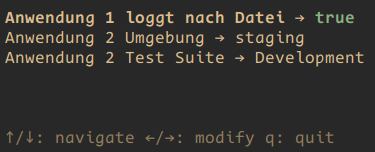
\includegraphics[scale=0.5]{post-start.png}}
    \end{center}
\end{figure}

\paragraph{Ansicht}
Abb. \ref{post-start} zeigt eine typische Ansicht direkt nach dem Start des
Programms. Die ersten drei Zeilen repräsentieren jeweils einen Eintrag in
der Konfigurationsdatei und somit eine Ziel-\gls{Textpassage} mit ihrem
aktuellen Wert. Jede dieser Zeilen besteht aus dem in der Konfigurationsdatei
vergebenen Titel des Eintrags, einem Pfeil und dem aktuellen Wert der Ziel-\gls{Textpassage}.
Die \textbf{aktuell ausgewählte Zeile} ist fett gedruckt während
\textcolor{teal}{der aktuelle Wert} der ausgewählten Zeile blau dargestellt wird.
Die genaue Darstellung ist dabei vom verwendeten Terminal-Emulator und dessen
Einstellungen bezüglich Schriftart und Farbwerten abhängig.

\paragraph{}
Die ausgegraute Zeile am unteren Rand beschreibt in Kurzform die verfügbaren
Kommandos und die davon ausgelösten Aktionen.

\paragraph{Aktionen}
Die Hauptfunktionen werden über die vier Pfeiltasten gesteuert. Die Pfeiltasten
hoch bzw. runter bewegen die Zeilenmarkierung nach oben bzw. unten. Die Pfeiltasten
links bzw. rechts schalten den zur markierten Zeile gehörigen Wert weiter zum
nächsten Wert aus der konfigurierten Liste der möglichen Werte
(siehe Kapitel \ref{Konfiguration} - Konfiguration). Beim Umschalten eines Werts
wird die zugehörige Zieldatei entsprechend modifiziert.

\paragraph{} Mit einem Tastendruck auf q kann das Programm jederzeit beendet werden
und zur Kommandozeile zurückgekehrt werden.

\subsection{Problembehandlung} \label{Problembehandlung}
\paragraph{Fehlende Konfigurationsdatei} Wenn beim Programmstart der Fehler
\begin{minted}[bgcolor=codebg]{bash}
    Error: No config file found at any of the search paths: ...
\end{minted}
auftritt, dann bedeutet das, dass bei der Suche nach Konfigurationsdateien an
keinem der angegebenen Pfade eine Datei gefunden wurde.
\paragraph{Lösung}
Es wird wie in Kapitel \ref{Konfiguration} (Konfiguration) beschrieben eine
Konfigurationsdatei an einem der validen Dateipfade angelegt. Im Dateisystempfad
unter

\begin{minted}[bgcolor=codebg]{bash}
    /usr/share/terminal-config-manager/config.yaml
\end{minted}

befindet sich eine Beispielkonfigurationsdatei, welche als Vorlage genutzt
werden kann:

\begin{minted}[bgcolor=codebg]{bash}
    mkdir ~/.config/terminal-config-manager
    cp  /usr/share/terminal-config-manager/config.yaml \
        ~/.config/terminal-config-manager
\end{minted}

\paragraph{Falsches Konfigurationsdateiformat} \label{missing-config} Wenn beim
Programmstart ein Fehler ähnlich

\begin{minted}[bgcolor=codebg]{text}
    An error occured while parsing the configuration file.
    The details are: ...
\end{minted}

auftritt, dann bedeutet das, dass die erste vom Programm gefundene Konfigurationsdatei
entweder nicht dem YAML-Format \cite{yaml} entspricht und/oder fehlende Elemente aufweist.

\paragraph{Lösung}
Die Fehlermeldung wird weitere Detailinformationen enthalten wie beispielsweise:

\begin{minted}[bgcolor=codebg]{text}
    The top level of the config file
    should be an object named 'config_lines_to_manage'
\end{minted}

anhand derer sich das Problem identifizieren lässt. Im Zweifelsfall muss dem
Kapitel \ref{Konfiguration} (Konfiguration) bzw. der Problembehandlung für
fehlende Konfigurationsdateien in Kapitel \ref{missing-config} folgend eine valide Konfigurationsdatei
per Hand angelegt werden.

\paragraph{Fehlende Dateizugriffsrechte} Wenn bei der Auswahl eines neuen Werts
der Fehler

\begin{minted}[bgcolor=codebg]{text}
    terminal-config-manager: <Zieldateipfad>: withFile:
    permission denied
\end{minted}

auftritt, dann bedeutet das, dass dem aktuellen Linux-Nutzer die nötigen
Zugriffsrechte fehlen, um die Zieldatei zu modifizieren.

\paragraph{Lösung}
Es muss sichergestellt werden, dass alle in der Konfigurationsdatei definierten
Zieldateien vom aktuellen Nutzer modifiziert werden können. Im häufigsten Fall
ist der aktuelle Nutzer nicht als \mintinline{bash}{owner} der Datei eingetragen:

\begin{itemize}
    \item Wenn dies angebracht ist, dann kann der Nutzer der Datei geändert werden:
          \begin{minted}[bgcolor=codebg]{text}
            chown <Nutzer> <Zieldateipfad>
        \end{minted}
    \item Wenn dies angebracht ist, dann können die Schreibrechte der Zieldatei
          angepasst werden:
          \begin{minted}[bgcolor=codebg]{text}
            chmod o+w <Zieldateipfad>
        \end{minted}
\end{itemize}

\textbf{Wenn keine der beiden oben genannten Optionen anwendbar ist, dann ist diese
    Zieldatei nicht für die Modifizierung durch das Programm geeignet}.

\newpage
\printbibliography

\newpage
\printglossaries

\end{document}